\chapter{Estadísticas y Métricas de Rendimiento}

Se detallan las métricas y estadísticas de rendimiento recopiladas durante las ejecuciones de prueba del generador de 
imágenes tipo \textit{cartoon}. Se describen los entornos de prueba, las configuraciones experimentales analizadas y se 
presentan los gráficos resultantes para visualizar el comportamiento de las distintas implementaciones paralelas.

\section{Métricas de Rendimiento}

Para evaluar y comparar cuantitativamente el desempeño de las implementaciones paralelas en relación con la versión 
secuencial de referencia, se utilizaron las siguientes métricas estándar:

\begin{itemize}
    \item \textbf{Tiempo de ejecución ($T_p$):} El tiempo total medido en segundos empleado en el procesamiento 
    de la imagen. Para garantizar la precisión de la medición del algoritmo en sí, este tiempo excluye las operaciones 
    de entrada/salida (I/O) en disco (carga de la imagen original y guardado del archivo final procesado).
    
    \item \textbf{Speedup o Aceleración ($S_p$):} Representa la ganancia de velocidad obtenida al utilizar recursos 
    paralelos en comparación con el algoritmo secuencial. Se define mediante la fórmula:
    \[S_p = \frac{T_1}{T_p}\]
    Donde $T_1$ es el tiempo de ejecución secuencial y $T_p$ es el tiempo de ejecución con la versión paralela 
    utilizando $p$ unidades de recursos (threads o procesos). Un speedup ideal sería igual a $?????$ (super lineal??).
    
    \item \textbf{Eficiencia Paralela ($E_p$):} Mide la fracción de tiempo durante la cual los procesadores asignados 
    son utilizados efectivamente para realizar cálculos útiles. Se define como:
    \[E_p = \frac{S_p}{p} = \frac{T_1}{p \cdot T_p}\]
    Una eficiencia de $1.0$ ($100\%$) indica que todos los recursos asignados están trabajando a su máxima capacidad 
    sin pérdidas por sobrecarga de sincronización, desbalanceo de carga o comunicación.
\end{itemize}

\section{Configuraciones Experimentales}

Las pruebas de rendimiento se llevaron a cabo variando múltiples parámetros del algoritmo y del entorno para analizar 
el comportamiento bajo distintas intensidades de cómputo y comunicación:

\begin{enumerate}
    \item \textbf{Resolución de las Imágenes:} Se utilizaron tres resoluciones con distinta cantidad de carga de trabajo:
    \begin{itemize}
        \item \textbf{Baja ($800 \times 800$ píxeles):} Carga de trabajo ligera ($640$ mil píxeles).
        \item \textbf{Media ($2000 \times 2000$ píxeles):} Carga de trabajo moderada ($4$ millones de píxeles).
        \item \textbf{Alta ($5000 \times 5000$ píxeles):} Carga de trabajo pesada ($25$ millones de píxeles).
    \end{itemize}
    
    \item \textbf{Intensidad del Filtro de Convolución (Borroneado):}
    \begin{itemize}
        \item \textbf{Filtro 3$\times$3 (Radio 1):} Requiere menor cantidad de operaciones por píxel.
        \item \textbf{Filtro 5$\times$5 (Radio 2):} Requiere mayor cantidad de operaciones de vecindad por píxel.
    \end{itemize}
    
    \item \textbf{Rangos de Posterizado:}
    \begin{itemize}
        \item \textbf{3 Rangos (Parámetro 1):} Pocos intervalos de discretización de color.
        \item \textbf{9 Rangos (Parámetro 2):} Mayor granularidad en el cálculo del color final.
    \end{itemize}

    \item \textbf{Recursos y Paradigmas Asignados:}
    \begin{itemize}
        \item \textbf{Secuencial:} Ejecución base con un solo thread/proceso ($1$ recurso).
        \item \textbf{OpenMP (Memoria Compartida):} Evaluado con 2, 4, 8, 16 y 32 threads en el cluster (y hasta 8 threads en local).
        \item \textbf{MPI (Memoria Distribuida):} Evaluado con 3, 8, 16 y 32 procesos en el cluster (y hasta 8 procesos en local).
        \item \textbf{Híbrido (MPI + OpenMP):} Evaluado en combinaciones de procesos $\times$ threads: $3\times2$, $3\times4$, 
        $3\times8$, $4\times8$, $8\times4$ y $16\times2$ en el cluster (y hasta $5\times2$ en local).
    \end{itemize}
\end{enumerate}

\section{Entornos de Ejecución}

Para contrastar el comportamiento del algoritmo bajo diferentes arquitecturas físicas, las pruebas se corrieron en dos entornos:
\begin{itemize}
    \item \textbf{Entorno Local (Prefijo CJ):} Ejecución sobre una máquina personal multiprocesador.
    \item \textbf{Entorno de cluster (Prefijo RC):} Ejecución sobre el cluster del departamento de informática, que permite evaluar el 
    rendimiento del paso de mensajes entre múltiples nodos de red físicos y la escalabilidad real en sistemas distribuidos.
\end{itemize}

\section{Visualizaciones de Desempeño}

A continuación, se presentan los gráficos generados para representar de manera sintética el comportamiento del sistema.

\subsection{Speedup Promedio por Configuración}
Las siguientes figuras muestran el Speedup promedio (calculado sobre todos los filtros y posterizados) clasificado por el tamaño de la imagen. 
Las configuraciones están ordenadas numéricamente para apreciar la progresión lógica de los recursos asignados.

\begin{figure}[H]
    \centering
    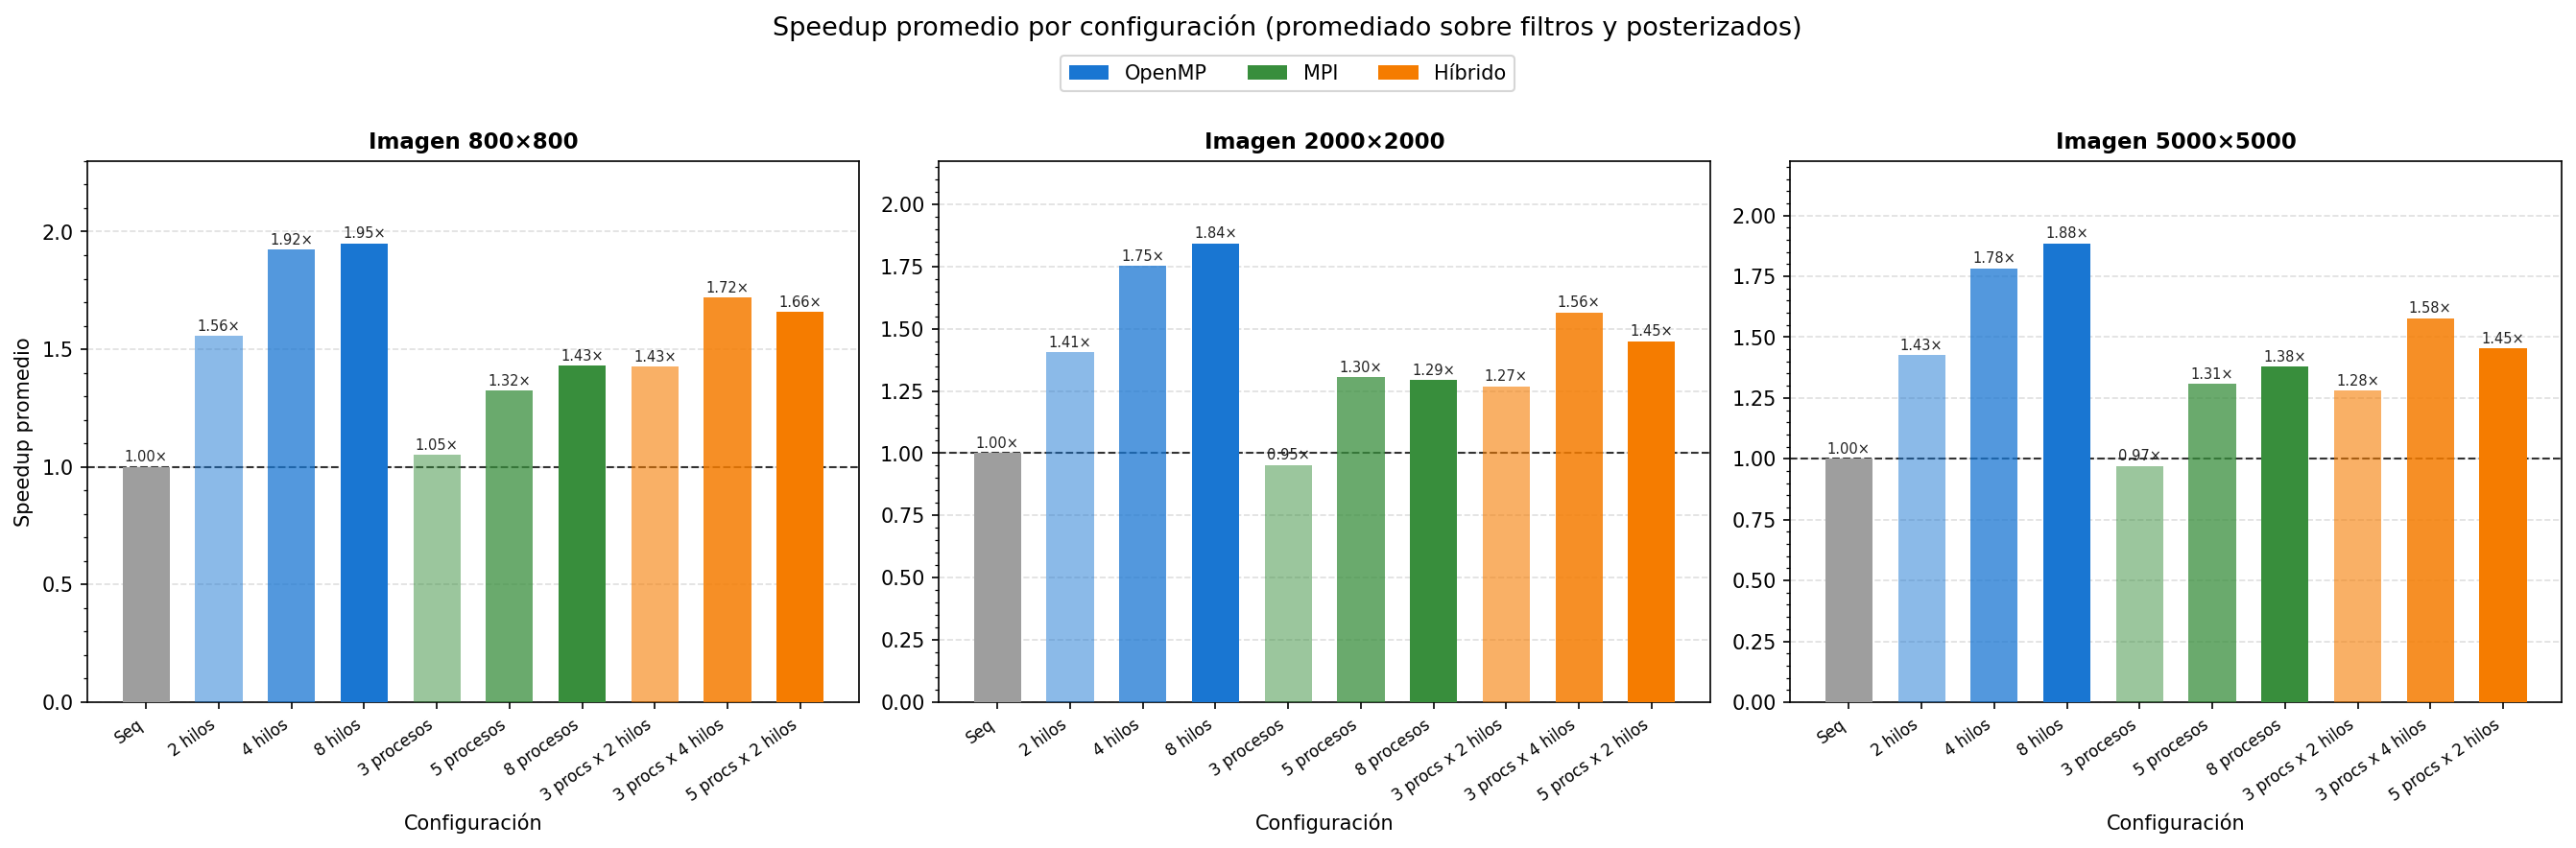
\includegraphics[width=0.95\textwidth]{../benchmark/graficos/CJ-1-barras_speedup.png}
    \caption{Speedup promedio por configuración en Entorno Local para imágenes de 800$\times$800, 2000$\times$2000 y 5000$\times$5000.}
    \label{fig:barras_speedup_local}
\end{figure}

\begin{figure}[H]
    \centering
    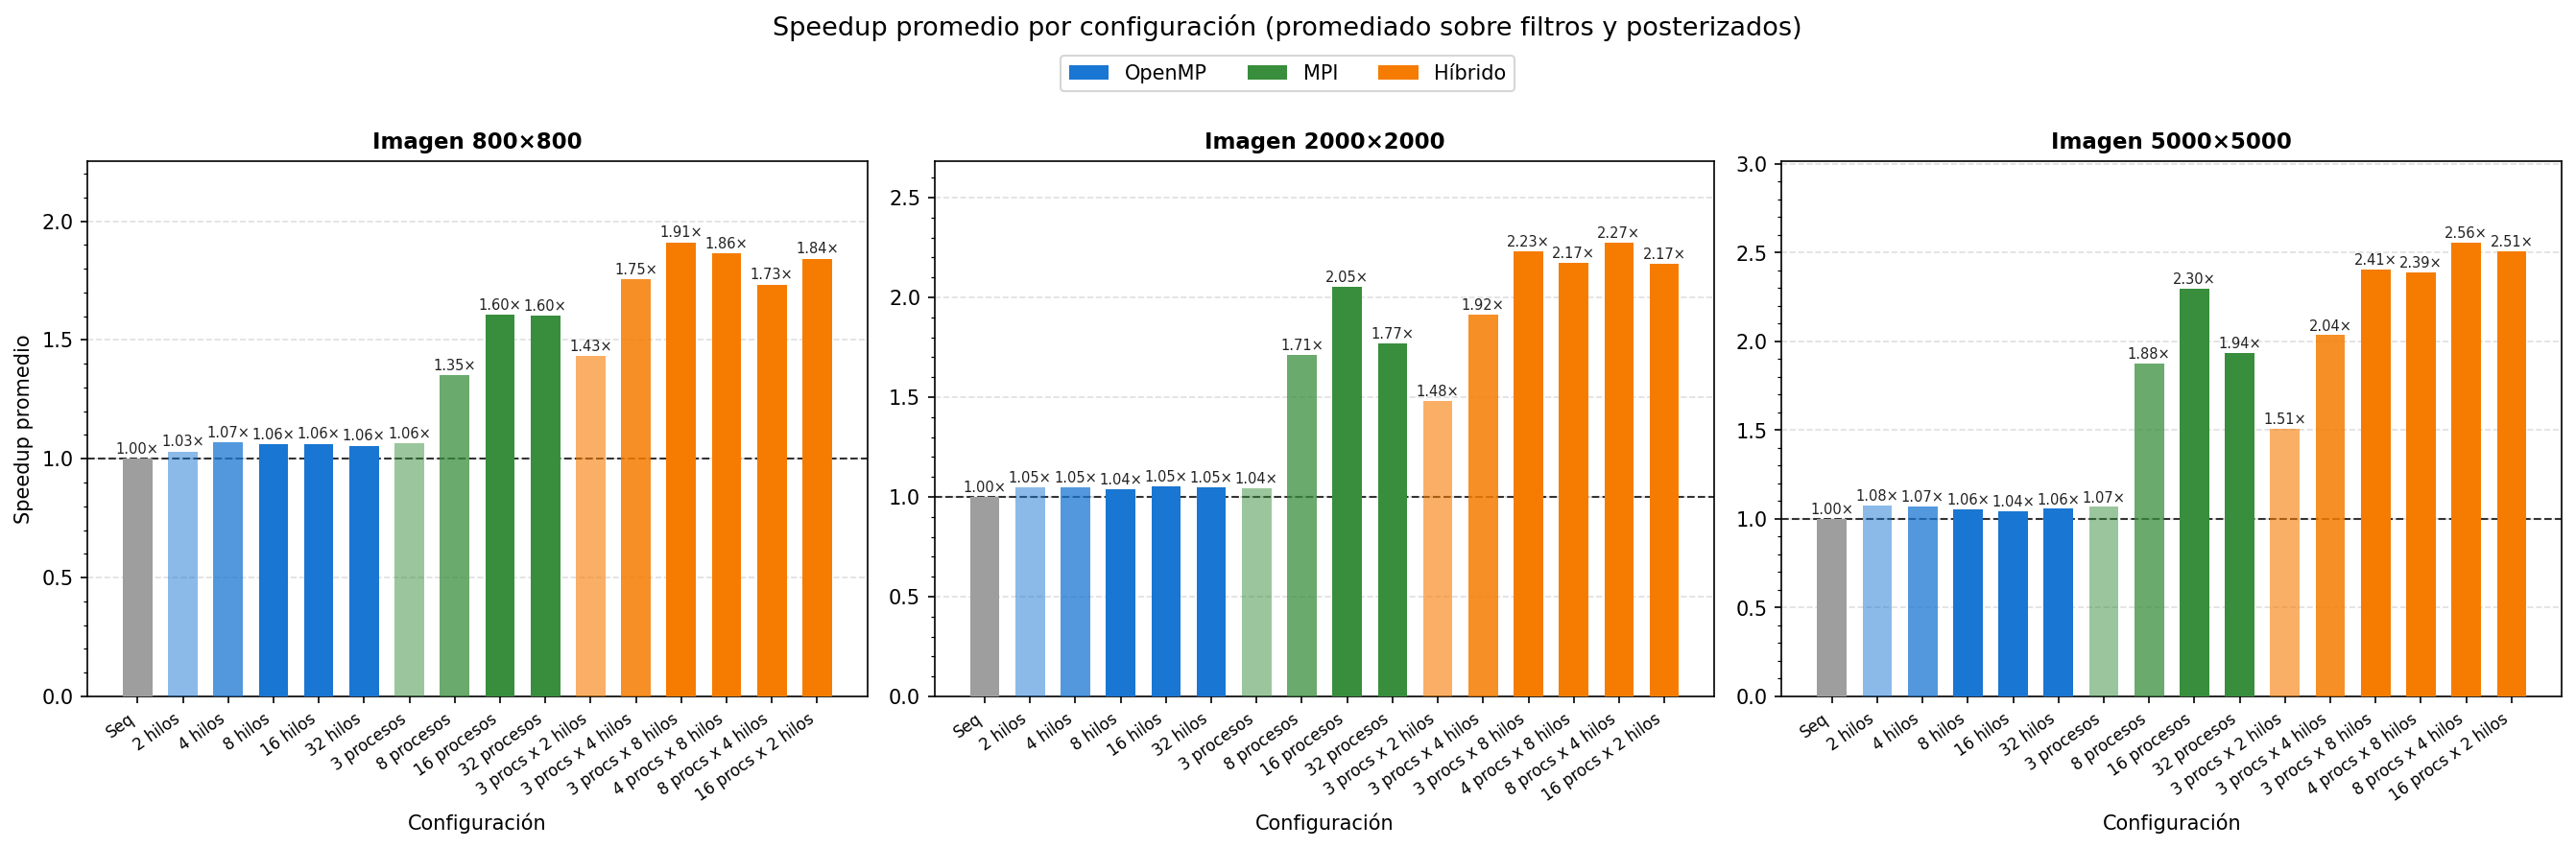
\includegraphics[width=0.95\textwidth]{../benchmark/graficos/RC-2-barras_speedup.png}
    \caption{Speedup promedio por configuración en Entorno cluster para imágenes de 800$\times$800, 2000$\times$2000 y 5000$\times$5000.}
    \label{fig:barras_speedup_cluster}
\end{figure}

\subsection{Eficiencia Paralela}
La eficiencia representa qué tan efectivamente se están usando los recursos agregados. El valor ideal es $1.0$.

\begin{figure}[H]
    \centering
    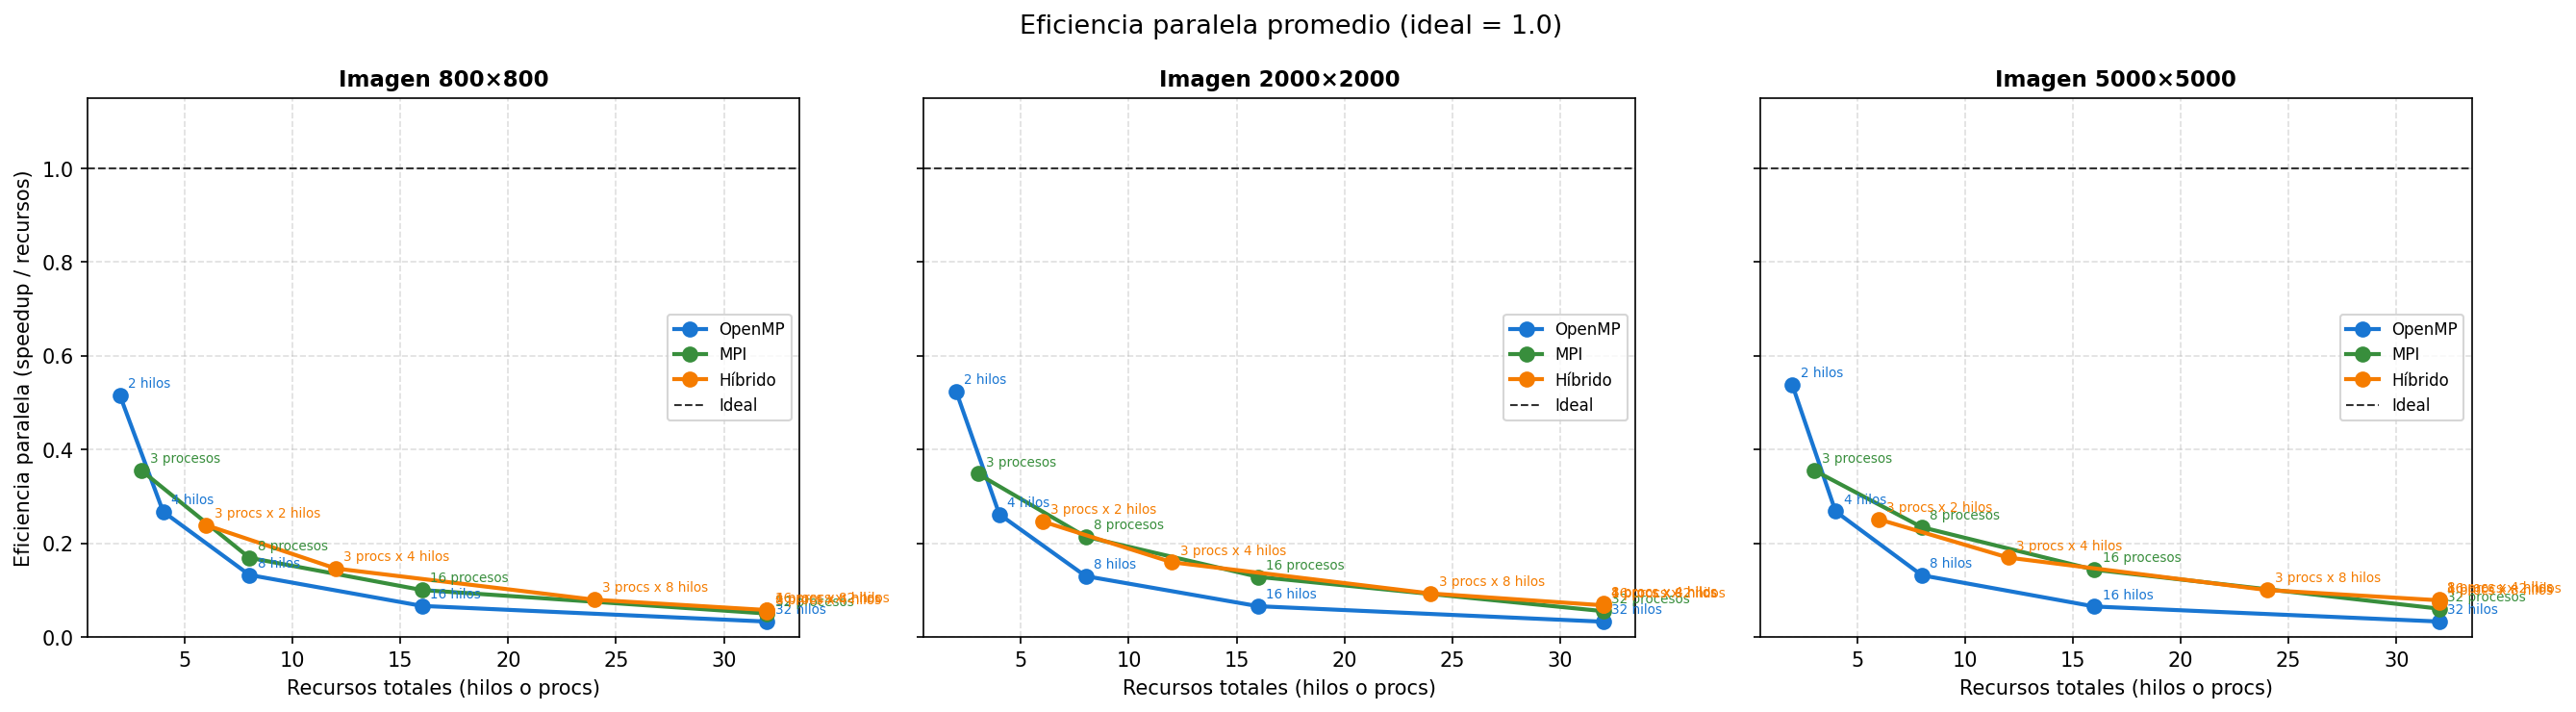
\includegraphics[width=0.95\textwidth]{../benchmark/graficos/RC-2-eficiencia.png}
    \caption{Eficiencia paralela promedio en Entorno cluster comparando OpenMP, MPI e Híbrido frente al comportamiento Ideal.}
    \label{fig:eficiencia_cluster}
\end{figure}

\subsection{Heatmap de Speedup por Escenario}
El heatmap permite cruzar todas las ejecuciones (combinaciones de resolución, filtro y posterización en el eje X) con todas las configuraciones de 
recursos (eje Y), mapeando el speedup absoluto en una escala de color.

\begin{figure}[H]
    \centering
    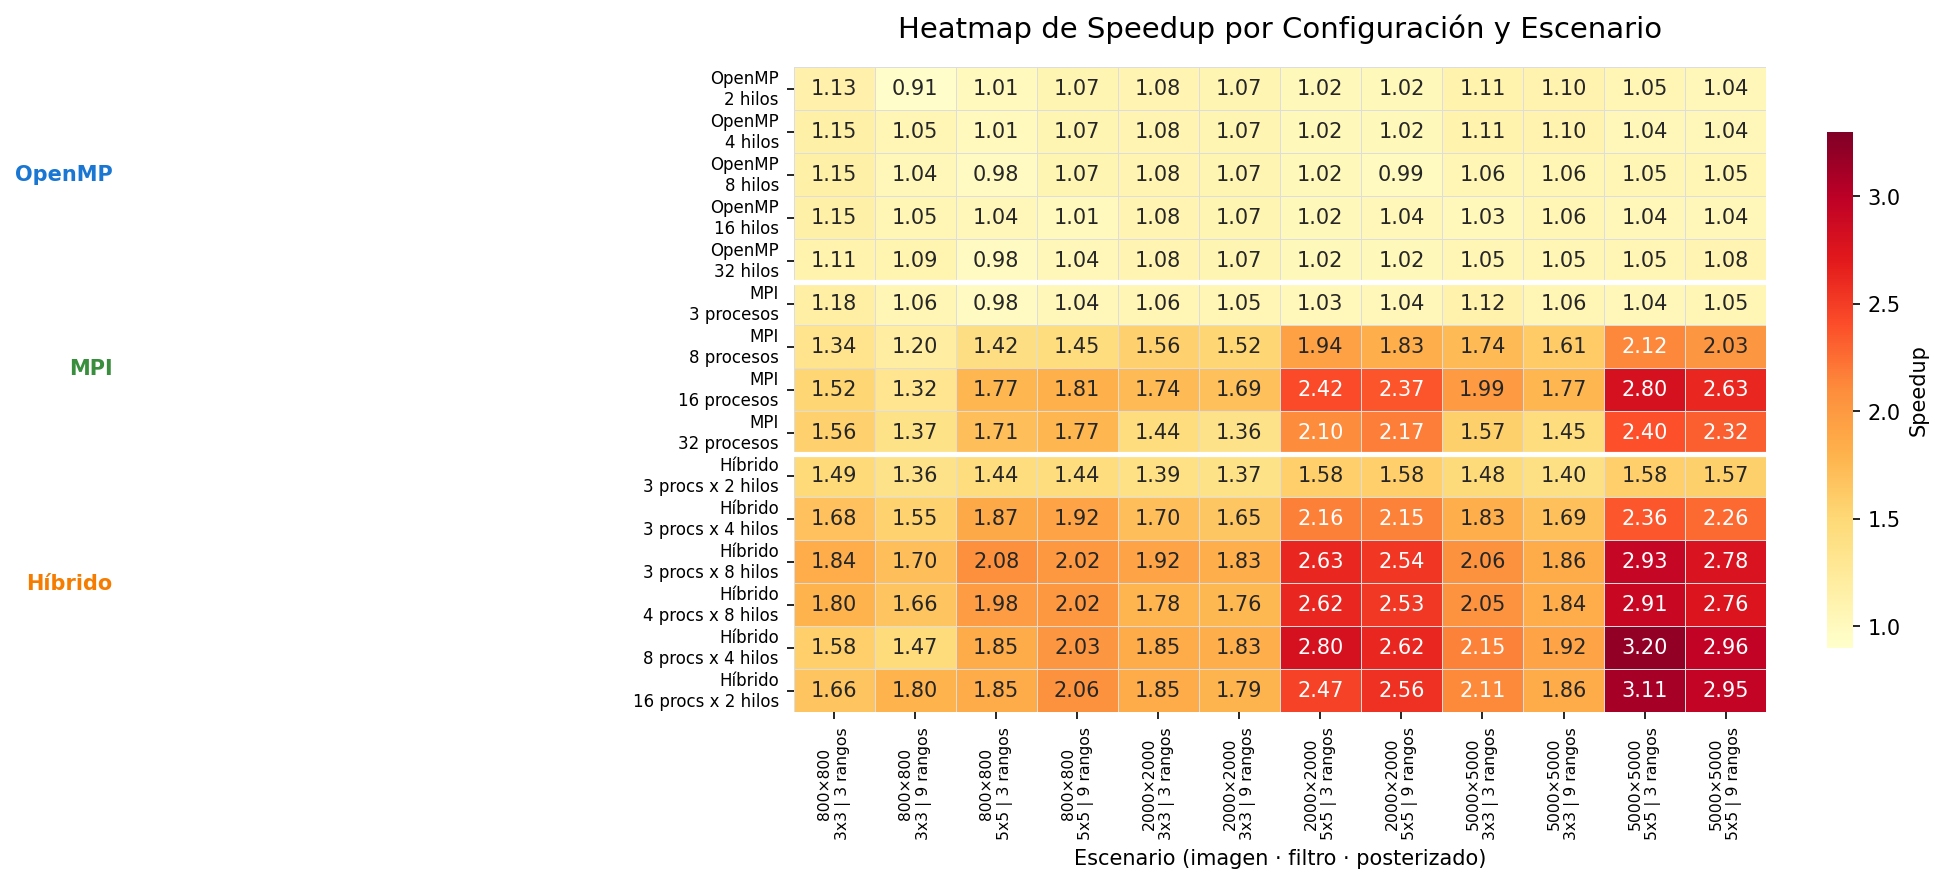
\includegraphics[width=0.95\textwidth]{../benchmark/graficos/RC-2-heatmap_speedup.png}
    \caption{Heatmap de Speedup detallado por escenario y configuración en el cluster.}
    \label{fig:heatmap_cluster}
\end{figure}

\subsection{Curva de Escalabilidad}
Muestra la evolución del speedup de la mejor configuración de cada paradigma a medida que el problema crece en volumen 
(de 800$\times$800 a 5000$\times$5000 píxeles).

\begin{figure}[H]
    \centering
    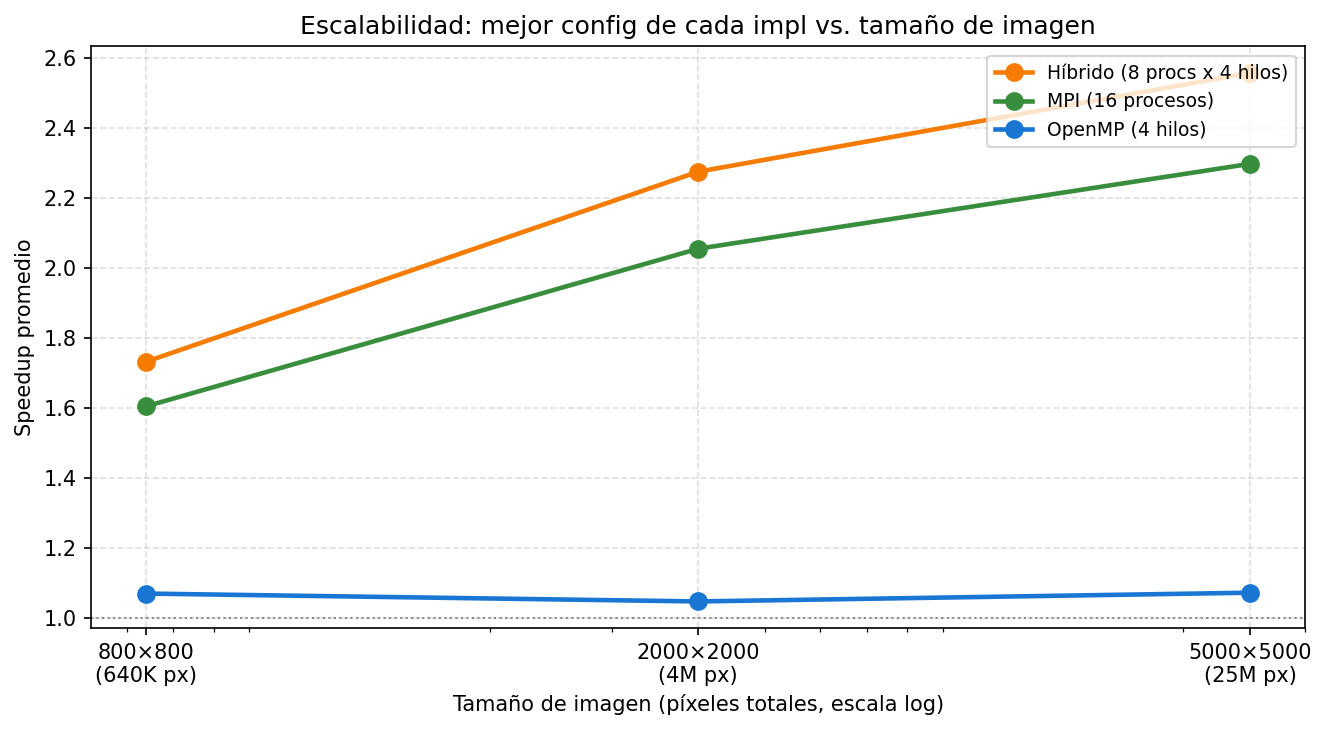
\includegraphics[width=0.8\textwidth]{../benchmark/graficos/RC-2-escalabilidad.png}
    \caption{Escalabilidad: Speedup promedio de la mejor configuración de cada implementación en función del tamaño de la imagen (cluster).}
    \label{fig:escalabilidad_cluster}
\end{figure}

\bigbreak
\noindent \textit{Nota: Las tablas numéricas de datos crudos obtenidas de cada ejecución se encuentran adjuntas en 
los Anexos \ref{appendix:local} y \ref{appendix:cluster} al final de este informe.}
